\section{Unit disk graphs}
\subsection{Properties}
\begin{frame}{Unit disk graphs}
  \begin{figure}
  \centering

  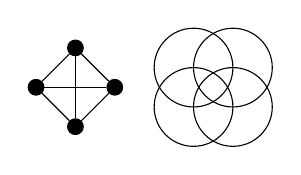
\begin{tikzpicture}

    \draw (-0.5,2.5) circle [radius=0.5];
    \draw (0,2.5) circle [radius=0.5];
    \draw (-0.5,2) circle [radius=0.5];
    \draw (0,2) circle [radius=0.5];


    \node[draw,circle,inner sep=2pt,fill,label distance=1cm] (v1) at (-2.5,2.25) {};

    \node[draw,circle,inner sep=2pt,fill,label distance=1cm] (v2) at (-2,1.75) {};
    \node[draw,circle,inner sep=2pt,fill,label distance=1cm] (v3) at (-2,2.75) {};
    \node[draw,circle,inner sep=2pt,fill,label distance=1cm] (v4) at (-1.5,2.25) {};

    \draw  (v3) edge (v2);
    \draw  (v4) edge (v1);
    \draw  (v3) edge (v1);
    \draw  (v4) edge (v2);
    \draw  (v3) edge (v4);
    \draw  (v1) edge (v2);

  \end{tikzpicture}

  \caption{Realization of a UDG.}
  \label{fig:udg}
  \end{figure}
\pause

\begin{theorem}
  CLIQUE problem is $\mathcal{NP}$-complete. Nevertheless, this problem is solved
  in polynomial time for unit disk graphs.
\end{theorem}

\pause
\begin{theorem}
  Unit disk graph recognition is $\exists \mathbb{R}$.
\end{theorem}
\end{frame}
